% 03.1. ASPECTOS ARQUITECTURALES Y TECNOLOGICOS
%----------------------------------------------------------------------------------------------
El patrón que utilizamos para el diseño arquitectural de nuestro catálogo electrónico es el de Modelo-Vista-Controlador, en concreto, la variante Modelo-Vista-Presentador del mismo (véase la~\cref{fig:diagDespliegue}).

\vspace{.2cm}
\begin{figure}[ht]
	\centerline{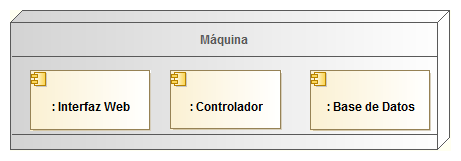
\includegraphics[scale=0.75]{img/diagrama_despliegue}}\
	\caption{Diagrama de despliegue del sistema}
	\label{fig:diagDespliegue}
\end{figure}
\paragraph{}
\paragraph{}
\noindent Los componentes de este diseño arquitectural son:

\paragraph{Interfaz web.} Es el componente que representa la vista de nuestra aplicación. Es el componente con el que los usuarios interactuan directamente para navegar por la aplicación y visualizar los resultados que producen las interacciones que realicen con la vista. Las acciones del usuario que impliquen el acceso a los datos del modeo o la modificación/eliminación de los mismos son delegadas al componente Controlador.

\paragraph{Controlador.} Es nuestro componente Presentador, tiene toda la lógica de la vista 
y es responsable de sincronizar el modelo y la vista. Es decir, cuando la vista notifica al 
Presentador que el usuario ha realizado alguna acción (por ejemplo, hacer clic en un botón) que afecta de alguna manera al modelo de datos del sistema, entonces el presentador se encarga de actualizar los datos pertinentes y sincronizar los cambios entre el modelo y la vista.

\paragraph{Base de datos.} Es nuestro componente modelo, se encarga de encapsular 
los datos y ofrecer operaciones para su acceso y procesamiento, es decir, ofrece persistencia de datos para la aplicación. Sólo el componente
Controlador interactúa con el modelo de datos..\newline\newline
Las tecnologías utilizadas son las que se detallaron en el apartado anterior.